\section{Protocol communication} \label{cha:protocolDesign}
To transmit the data from the sensor nodes to the main node, a protocol will be implemented. The protocol is built to be hardware independant, and should thereby work on other components than the ones chosen for the solution.

% Background/meta
The protocol to be developed for the solution will be based on the networks examined in chapter \ref{cha:networksprot} and protocols examined in chapter \ref{cha:comprot}.
There are a number of considerations to be made to develop a protocol that statisfies the requirements.
Because the sensor nodes are battery driven, most of the choices are done with power consumption as a priority, to increase the battery longevity.

% Range limitations
A restriction of the radio modules is their relatively short communication range. The reach of the system can be extended by introducing relaying, so that a sequence of nodes can interconnect and transfer data through the branch in the tree. Therefore, relaying must be supported by the protocol as stated in chapter \ref{cha:requirements}. 

% Other limitations and considerations
% To fulfill the requirements found in \ref{cha:requirements}, there is no demand to request data for only one specific node at a time.

The radio modules selected for the solution are half-duplex and not capable of full-duplexing, and this limitation needs to be addressed in the development of the protocol. 

% Already mentioned in design intention/data handling => move?
For power consumption and complying to the usage, the network nodes are controlled by the main node, and the sensor nodes will only transmit data on demand. There is no requirement for real-time monitoring of the golf course, making it difficult to define a data transfer interval that matches both power consumption as well as the need for information.
Hence, an on-demand request for data is be sufficient.

\subsection{Packet Transfer}
% Intention/motivation
The solution is developed to gather sensor data from all nodes in a network, and this subsection will contain the considerations regarding choice of transfer method and the according topology.

%This enables the main node to broadcast data requests throughout the sensor network, and likewise transmitting data readings from the sensor nodes to the main node.

% The two types of communication (data request and data respond)
As the sensor readings are required on-demand, there must be at least two types of communication. The first being the data request; an outgoing signal from the main node, notifying the sensor nodes of the data demand. This is a broadcasted packet, as every node is targeted as recipient. The second type is data response, as the sensor readings needs to be returned to the main node for storage and representation.

% Design of data request: individual request
Sending individual requests is not appropriate as routing tables would use a significant amount of the limited memory of the network nodes, if the addressee is a sufficient amount of nodes away. In case of disconnected nodes, the routing tables must be reconfigured, to make sure packets are relayed in a path that actually exist and is within range. This would accordingly require nodes to somehow broadcast that they are still alive, and thereby consume more energy in addition to more memory usage.

% Data request method selection template
The protocol used in the solution is partially based on the controlled flooding protocol, as described in chapter \ref{cha:floodingSec}.
This protocol is a method where the data request can be transmitted by flooding the network, without the need of sending a tailored request to every node in the network. 

The controlled flooding has a low memory impact and thus best suited for the solution. The flooding protocol will create a tree which can be utilized to create a return path for the sensor readings of the sensor nodes.

% Practical implementation of data request
\begin{figure}[h!]
	\centering
	\makebox[\textwidth][c]{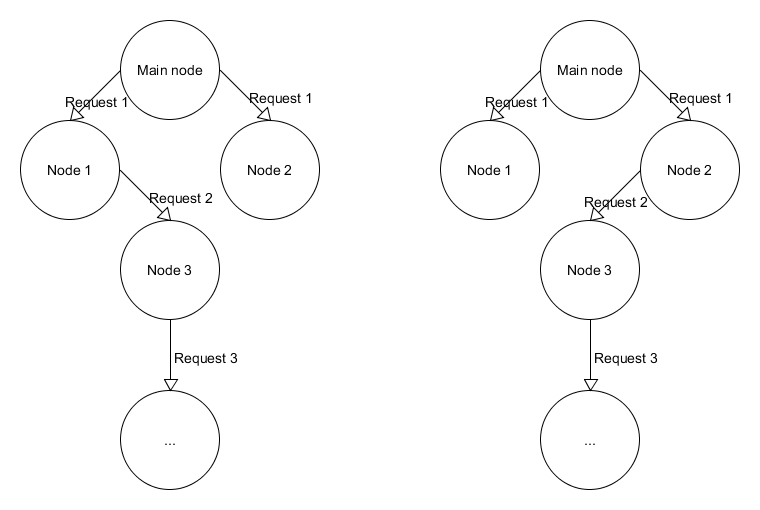
\includegraphics[scale=0.4]{chapters/design/figures/branchExample.png}}
	\caption{The tree structure can vary depending on the node that gets a reuqest to a subnode first.}
	\label{fig:treeVariation}
\end{figure}

The tree created, in each wave of request broadcasts, can vary in its structure, depending on interference, removal of nodes, or faulty nodes. Figure \ref{fig:treeVariation} shows an example of how the tree can vary: first the main node will broadcast \textit{request 1}, which is received by both \textit{node 1} and \textit{node 2}. A sensor node in the system will always handle its own sensor data before relaying data from other nodes. If the main node receives sensor data from \textit{node 1} first, the resulting tree will match the tree seen to the left in \figref{treeVariation}. If \textit{node 2} connects to the main node first, the tree will match the tree seen on the right.
This will effectively solve the requirement of responding appropriately to a disconnecting node, as well as the inclusion of new nodes in the network, since a new tree is constructed with each new requests from the main node.

% Design of data respond
In other words, a tree instantiated by the controlled flooding protocol can be used to construct a tree that spans over a single path from each node to the main node.
The receiver of a request signal can use the sender as the parent when data is to be returned.
The subnode will then repeat the request signal, and be the parent of nodes hearing it.
Any node receiving a request signal will then be able to respond to its parent, causing all nodes to have a single identifier for the routing towards the main node.

%\subsection{Overloaded nodes}
Observe that nodes close to the main node are prone to receive a large amount of data since many, if not every, data packet must go though that node. Looking at figure \ref{fig:prottree1} it is shown that \textit{node 2} will handle every data packet on the path to the main node. Such low level nodes might be overloaded with data packets, causing a bottleneck if not thoughtfully spread out. The risk of collisions rise if several higher level nodes are trying to send data packets back to \textit{node 2}, but \textit{node 2} has a limited packet throughput. Another scenario is that since \textit{node 2} is relaying data more frequent than other nodes in the system, it consumes more energy and could  run out of power before subnodes. This could result in the loss of an entire branch.

\subsection{Sequence}
In this subsection the sequence of how the main and sensor nodes behaves after receiving a packet will be described.
The general sequence of the protocol is determined as the flowchart seen in appendix \ref{cha:flowchart}.

The following is the operation structure for each individual node in the system.

\textbf{Sensor nodes} \\
\begin{enumerate}
\item If the node have not yet been paired up with the main node.
	\subitem Send a pair request to the main node.
	\subitem Await acknowledgement from the main node and remember the assigned ID.

\item Receive a data request and remember the addresser as parent.

\item Acquire data from sensor and send it to parent.
\subitem Await acknowledgment from parent.
	\subsubitem Resend data if no acknowledgement is received.

\item Generate and broadcast request.

\item Await data from subnodes.
	\subitem Respond to subnodes with acknowledgement.
	\subitem Received data is relayed to parent.
	
\item If no response or acknowledgment within timeout limit is received, or a clear signal have been received: clear all data except its own ID, relay the clear signal, and await new data request.
\end{enumerate}


\subsubsection*{Main node}
\begin{enumerate}
\item When receiving pair request, assign and save ID for the requesting node and respond with an acknowledgement containing the ID.
\item When the greenkeeper requests data in the interface, broadcast a data request.
\item When receiving data from a subnode, save the data and respond with an acknowledgement to the subnode.

\item When data have been received from all registered nodes, broadcast a clear signal and show the data for the greenkeeper.

\item If the timeout limit is reached without being finished, the data is sent and a clear signal is broadcasted.
\end{enumerate}



\subsection{Interference handling} \label{cha:crcDesign}
When utilizing wireless communication, interference can be a problem, as explained in chapter \ref{cha:dutuVurufucutiun}. This is also the case when using controlled flooding, but the protocol can potentially help reduce problems with interference, for instance by validating the transferred data and acting accordingly.

Interference might cause a change in a packet, which will make the received data unusable. Figure \ref{fig:prottree1} shows an example of a possible interference scenario, where nodes 5, 6, and 7 could send packets at the same time, causing node 3 to receive scrambled data.

To counteract this problem, a checksum is used for verifying packets. This checksum is transmitted with the data and recipient. When a node receives a packet, the checksum is calculated, hence verifying the contents of the packet. How the checksum is calculated is explained in section \ref{cha:crcComp}.

To ensure that a packet eventually is received, the nodes will wait a random, but progressively longer, interval, between attempting to send data. This increases the chances for the transmitted data to reach the receiver without interference. Exponential backoff is further explained in chapter \ref{cha:expbackoff}.

%\subsection{Data importance}
It should be noted that the monitored data is not critical. If a packet is lost, it is negligible. If data is not received from one or multiple sensor nodes, a new request can be sent or the node can be repaired or replaced.
%If the user of the system discovers missing data from a certain area or node, the node can be fixed or replaced.


\subsection{Summary}
The protocol uses flooding to distribute the data request through the network. 
When data is requested by the user, the main node sends a packet containing a data request. 
The nodes that receive this packet directly from the main node is the first level of nodes in the tree, as seen in figure \ref{fig:prottree1}. 
These nodes then read the moisture values from their sensors and transmit these back to the main node. 

The first level nodes then request data from the nodes within their range. 
The nodes receiving this request firstly verifies that it is a new request, then registers the node that requested data as its parent. 
These nodes are second level nodes. The second level nodes read from the sensors, and sends data back to their parents. The parents then relay the data to the main node. 
This procedure continues until all reachable sensors have relayed data back to the main node.
An illustration showing an example of a tree is seen on figure \ref{fig:prottree1}.

For each new data request from the main node the tree structure and node levels are assessed again as they might have changed, due to new or disconnected nodes.

\begin{figure}[!h]
	\centering
	\makebox[\textwidth][c]{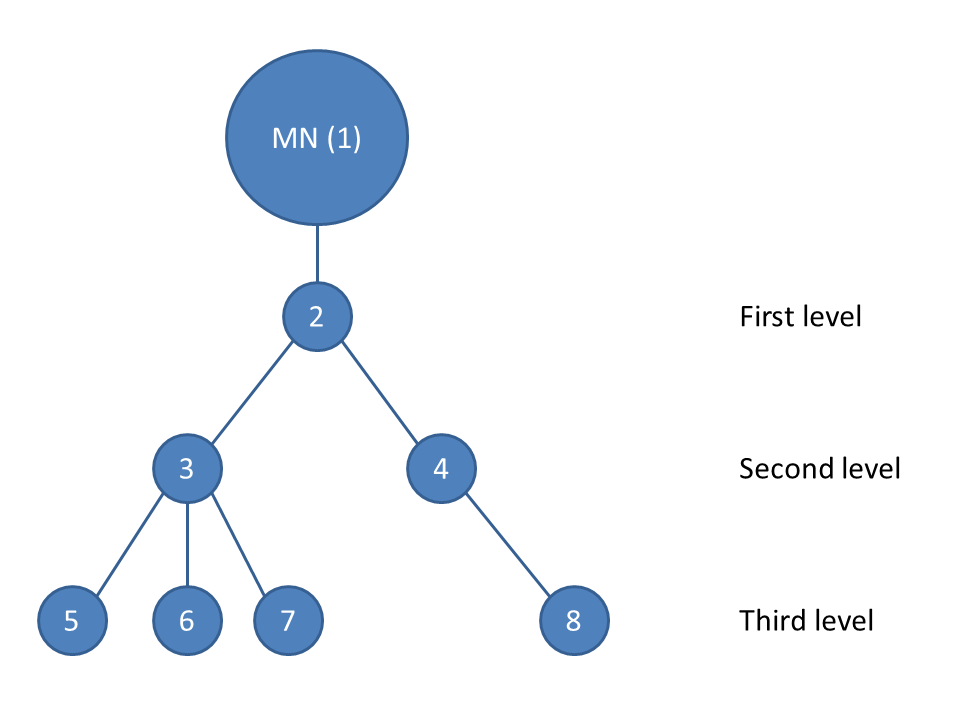
\includegraphics[width=1\textwidth]{chapters/design/figures/prottree1.png}}
	\caption{Example of a tree.}
	\label{fig:prottree1}
\end{figure}


\section{Packet}
This section covers the descriptions and decisions regarding the packets sent wirelessly in the network.

\subsection{Packet types}
% Motivation
To be able to discern and utilize received data, it is decided to mark the packet accordingly, indicating the packet content.
The types are used to inform the receiver what type of data the packet contains, so that the receiving node can decide how to handle the received packet. 

% Limitations
There are multiple types of data used in the protocol. As the solution is modular, the protocol is supposed to support other modules; also modules only capable of smaller packet sizes. Though, a packet size of 16 bytes is required to contain the necessary data from the nodes.

% Meta
Below is a description of the different packet types:

\textbf{Data}\newline
The \textit{data} packet fulfills the main requirement of transmitting the sensor readings to the main node.

\textbf{Data request}\newline 
The \textit{data request} packet is the packet notifying the receiving nodes of a data demand. 
The packet contains the transmitting the ID of the node, so that sensor nodes receiving the packet knows the sender, thus enabling the receiving nodes to set a parent ID. 

A lifespan variable is also contained in this packet, used for determining when to stop relaying requests. When the main node requests data, the contents of lifespan is the number of known nodes in the network. The lifespan variable gets decremented by one with every relay. This prevents potential request loops.

\textbf{Data acknowledgement}\newline
A \textit{data acknowledgment} packet is used to confirm that the sent \textit{data} packet has been received correctly. The parent node is responsible for sending a \textit{data acknowledgment} to the addresser of the received packet. 

\textbf{Pair request}\newline
A \textit{pair request} packet is sent by an unregistered sensor node and handled directly by the main node, which means it must be within range of the main node. The purpose is to assign an ID to the sensor node, so that every sensor node is registered in the system. The ID's enables the main node to confirm that data is collected from all sensor nodes for the current data gathering, and to identify the origin of the collected data. The ID also provides the capability of a parent-child hierarchy.

\textbf{Pair request acknowledgement}\newline
The \textit{pair request acknowledgement} packet is sent by the main node and used to confirm that the \textit{pair request} has been received and accepted. A \textit{pair request acknowledgement} packet also contain the ID that have been assigned to the specific node. When the two nodes, main and sensor node, are paired, the sensor node can then be deployed on the golf course. 

\textbf{Clear signal}\newline
The \textit{clear signal} is used to reset every node in the network, which will happen once the main node have received data from all registered nodes in the system.
The \textit{clear signal} packet lets every node in the network know that it should forget any previous information stored, except its own ID. This is done to add flexibility to the system. When \textit{data requests} spread through the network, it forms a tree based on how the nodes are placed. By resetting with the \textit{clear signal}, a new tree could be created each time a new wave of \textit{data requests} goes through the network, which in turn means that nodes can be moved around the golf course between waves of \textit{data requests}.

\textbf{Error}\newline
Because packets are not always transferred correctly, the receiver node will verify the integrity of a packet whenever a packet is received. Section \ref{cha:crcDesign} describes how this is done. If the checksums do not match, the packet type will be set to \textit{error} and discarded.

% Adresses
\subsection{Addresses}
The packet contains the addresser, addressee and the origin address which can be seen in figure \ref{fig:dataalloc}. Due to the potential number of sensor nodes in the network, atleast 2 bytes is required for each address.

\textbf{Addresser}\newline
When a node receives a packet, for instance a packet of the \textit{data request} type, the node needs to respond with its sensor data. The node could begin broadcasting its sensor data openly as response, however this could potentially be received by other nodes in range, whereas the sensor data might be irrelevant. This is why a packet contain the ID of the sender, which is the addresser. The addresser address gives the node knowledge of which node requested data and can therefore address its data correctly. Other nodes in range might receive the data as well, but they will ignore the packet since it was not addressed for them.

The addresser field of a packet will change during the packets lifetime. This happens when a node forwards a packet from another node. The addresser ID will be replaced by the ID of the node relaying the data.

\textbf{Addressee}\newline
When a node wants to send a packet with its sensor data, a data type packet in this case, it need to specify who this data is meant for, which is the node that requested the data. The ID of the node that requested the data will be marked in the packet as the addressee. This is done to ensure that the packet reaches the intended node. When a node, that is expecting a data packet, receives such a packet, it compares the addressee of the packet with its own ID. The packet will be ignored by the node if the addressee and the ID of the sensor node do not match.

The addressee field of a packet will change during the packets lifetime. This is the case when the packet is relayed, in the same way that the addresser changes.

\textbf{Origin}\newline
The origin contains the ID of the node where the data of a specific packet originated. This data is used by both the main node and the external nodes to differentiate the data.

The origin field of a packet will not be altered during the lifetime of the packet.


\subsection{Data}
When a data packet is constructed, the sensor data is stored in the "data" blocks of the packet as seen in figure \ref{fig:dataalloc}. There are three blocks available for sensor data storage. The solution will, at this time, only contain an implementation of the moisture sensor, but the aim of the three data fields is to add extendibility by enabling support for a maximum of tree sensors per node, each with its own field in the packet.


\subsection{Checksum}
There is a possibility that a packet is not transferred correctly. The packets checksum is stored in the checksum field of the packet and is used for verification.


\subsection{Packet allocation}
The limitation of the network size is 1000 nodes. This means the addresser, addressee and origin address fields need to support 1000 unique addresses, which requires 9 bits. The allocated size for the addresses are accordingly 2 bytes(16 bits) each to maintain usage of whole bytes. This is done because it is more efficient to manipulate a byte instead of bits \cite{bytevsbit}. The addresses requires 6 bytes in total.

The readings of the moisture sensor have a range of 1024 values, and the required size allocated for the sensor reading data is 10 bits. The allocated data size in the transfer is therefore 2 bytes.

The sizes of the different data to transfer sums up to 16 bytes and the distribution is displayed in figure \figref{dataalloc} as the data 1, data 2, and data 3 fields.

\subsection{Verification of a packet}
%Verification of a message
The received packet is verified by generating a checksum of message $m$ plus previously generated checksum $r$.
The new generated checksum of a correctly transferred packet $T$ is 0, because a package $T$, if correctly transferred, is some quotient $Q$ times the polynomial $G$, as seen in \charef{crcComp}. If a division has a zero remainder, the packet was transferred correctly.


The nRF24L01 supports data payloads up to 32 bytes. Only half of the space available in a transmission is actually occupied. The packet overview can be seen in \figref{dataalloc}, where each block represents 1 byte.
\begin{figure}[h!]
	\centering
	\makebox[\textwidth][c]{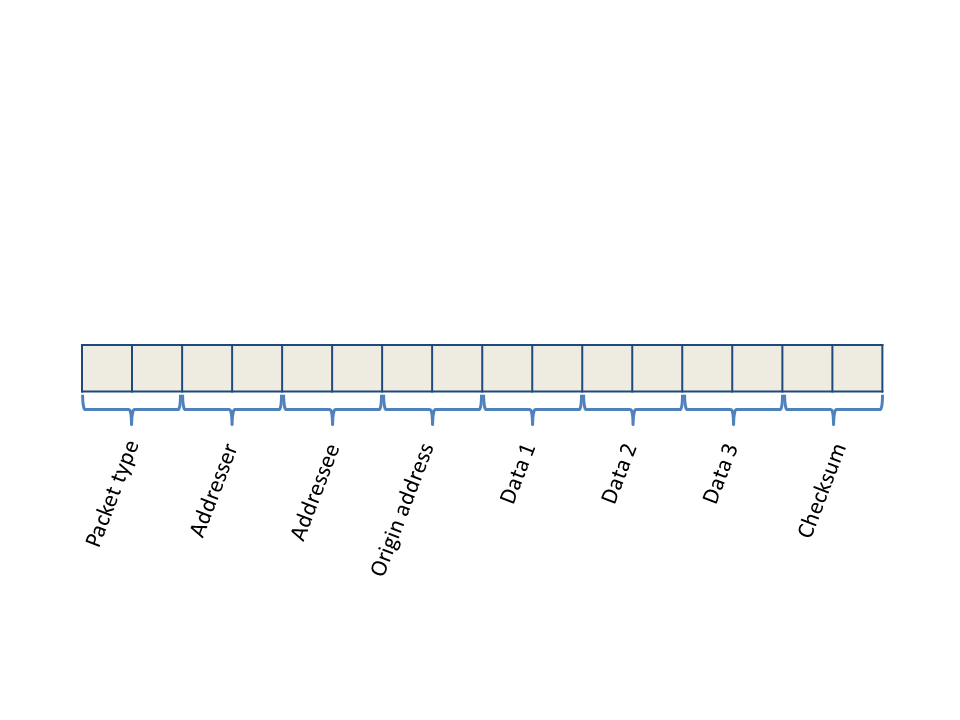
\includegraphics[width=1\textwidth,trim={0 3cm 0 8cm},clip]{figures/dataalloc.png}}
	\caption{Data allocation in packets, where each slot is 1 byte.}
	\label{fig:dataalloc}
\end{figure}

\subsection{Adding and removing nodes}
If a new node is to be added to the network, it needs an identifier in the system so that its sensor reading can be recognized. The identifier is permanent as long as it is in the network.
The identifier is provided by the main node by pairing the device with the main node. 

Should a node somehow disconnect from the network, the nodes connected to this node will receive the packets from another node instead, and from that point on use that as the parent. This is valid if there are any nodes in range of the disconnected children of the nodes. 
